
\documentclass[11pt]{amsart}
\usepackage{geometry}                % See geometry.pdf to learn the layout options. There are lots.
\geometry{letterpaper}                   % ... or a4paper or a5paper or ... 
%\geometry{landscape}                % Activate for for rotated page geometry
\usepackage[parfill]{parskip}    % Activate to begin paragraphs with an empty line rather than an indent
\usepackage{graphicx}
\usepackage{amssymb}
\usepackage[all]{xy}
\usepackage{epstopdf}
\DeclareGraphicsRule{.tif}{png}{.png}{`convert #1 `dirname #1`/`basename #1 .tif`.png}


% these packages make it easy to include figures in the text. 
\usepackage{float}
\restylefloat{figure}

\newcommand{\cX}{\mathcal{X}}
\newcommand{\cC}{\mathcal{C}}
\newcommand{\cF}{\mathcal{F}}




\begin{document}
{\Large Name: Philip Pham}  \\
\begin{center}
\Large AMATH 515 \hskip 2in Homework Set 1\\
{\bf Due:  Monday Jan 27th, by midnight}. 
\end{center}
\bigskip
\begin{enumerate}

%\item Read section 1.5 of the course notes (LivingText) and show the following: 
%\begin{enumerate}
%\item First part of Corollary 1.14. Given any $\beta$-smooth function $f: U \rightarrow \mathbb{R}$, for any points $x,y \in U$, the inequality 
%\[
%\left| f(y) - f(x) - \nabla f(x)^T(y-x)\right| \leq \frac{\beta}{2}\|y-x\|^2
%\]
%holds. 
%
%\item In class we saw that the operator norm on $\nabla^2 f(x)$ gives a $\beta$. Show the opposite direction, i.e. that if $f$ is $\beta$-smooth 
%and twice-continuously differentiable, then $\|\nabla^2 f\| \leq \beta$.
%
%\end{enumerate}
%
%\bigskip\bigskip

\item Show that if $g:\mathbb{R}^m \rightarrow \mathbb{R}$ is a twice differentiable function,  $A \in \mathbb{R}^{m\times n}$ any matrix, 
and $h$ is the composition $g(Ax)$, then  
\begin{enumerate}
\item $\nabla h(x) = A^T \nabla g(Ax)$.

  Use $D$ for the total derivative rather than abuse the $\nabla$ notation. If
  $f: \mathbb{R}^n \rightarrow \mathbb{R}^m$, then the linear map
  $D_a f: \mathbb{R}^n \rightarrow \mathbb{R}^m$ is the total derivative of $f$
  evaluated at $a$. With this definition, for functions,
  $f: \mathbb{R}^n \rightarrow \mathbb{R}$, we have that
  $\left(D_x f\right)^T = \nabla f (x)$.
  
  \begin{proof}
    
    Clearly, \begin{equation*}
      \lim_{h \rightarrow 0} \frac{A(x + h) - Ax - Ah}{h} = 0, \forall x \in \mathbb{R}^n
    \end{equation*}
    since $A$ is a linear map. Thus, by definition $D_x A = A$.

    The chain rule tells us that if $F(x) = G(H(x))$, then
    $D_x F = D_{H(x)} G \circ D_x H$. In this case, the composition operator is
    just matrix multiplication. We have that
    \begin{equation*}
      D_x h = D_{Ax} g \circ D_x A = D_{Ax} g \circ A,
    \end{equation*}
    which implies that
    \begin{align*}
      0
      &= \lim_{h \rightarrow 0} \frac{g(A(x + h)) - g(Ax) - \left(D_{Ax} g \circ A\right)h}{h} \\
      &= \lim_{h \rightarrow 0} \frac{g(A(x + h)) - g(Ax) - \langle A^T\left(D_{Ax} g\right)^T, h \rangle}{h} \\
      &= \lim_{h \rightarrow 0} \frac{g(A(x + h)) - g(Ax) - \langle A^T\nabla g(Ax), h \rangle}{h}.
    \end{align*}
    Thus, by definition, $\nabla h(x) = A^T \nabla g(Ax).$
  \end{proof}
\item $\nabla^2 h(x) = A^T \nabla^2 g(Ax) A$
  \begin{proof}
    Define $F(x) = A^T\nabla g(Ax)$, so
    $F: \mathbb{R}^n \rightarrow \mathbb{R}^n.$ We can apply the chain rule again:
    \begin{equation*}
      D_x F = A^T D_x  \nabla g(Ax) = A^T \nabla^2 g(Ax) D_xA = A^T \nabla^2 g(Ax) A.
    \end{equation*}
    Since $D_x F = \nabla^2 h(x)$, we have our desired result.    
  \end{proof}
\item Use the formulas to compute the gradient and Hessian of the logistic
  regression objective:
\[
\sum_{i=1}^n \log(1+\exp(\langle a_i, x\rangle))- b^TAx
\]
where $a_i$ denote the rows of $A$.

\begin{proof}
  We can write the terms in the summation as $g(a_i^Tx)$, where
  $g(x) = \log(1 + \exp(x))$. We have that
  \begin{align*}
    \nabla g(x) &= \frac{\exp(x)}{1 + \exp(x)} \\
    \nabla^2 g(x) &= \frac{\exp(x)}{\left(1 + \exp(x)\right)^2}.
  \end{align*}

  Let
  \begin{equation*}
    l(x) = \sum_{i=1}^n \log(1+\exp(\langle a_i, x\rangle))- b^TAx.
  \end{equation*}
  Applying the previous results to each term, we obtain
  \begin{align*}
    \nabla l(x) &= \sum_{i=1}^n a_i\frac{\exp(\langle a_i , x \rangle)}{1 + \exp(\langle a_i , x \rangle)} - A^Tb \\
    \nabla^2 l(x) &= \sum_{i=1}^n a_ia_i^T\frac{\exp(\langle a_i , x \rangle)}{\left(1 + \exp(\langle a_i , x \rangle)\right)^2}.
  \end{align*}
\end{proof}
\end{enumerate}

The point here is just to show why these formulas hold. One way to proceed is to be fully explicit in all coordinates but this is time consuming and not very insightful. A better way to go is to think about efficient ways to write the 
product $Ax$ that makes it easy to differentiate with respect to each coordinate. 


\bigskip\bigskip


\item Explain why each of the following functions is convex. 

\begin{enumerate}
\item Indicator function to a convex set: 
\(
\delta_C(x) = \begin{cases} 0 & \mbox{if} \quad x \in C \\ \infty & \mbox{if} \quad x \not \in C. \end{cases}
\)

\begin{proof}
  This follows from the defintion that
  $$f(\lambda x + (1-\lambda)y) \leq \lambda f(x) + (1 - \lambda)f(y)$$ for all
  $x$ and $y$ and $\lambda \in [0, 1]$. We have four cases: (1) if $x \in C$ and
  $y \in C$, then both the left-hand side and right-hand side are always $0$ and
  the inquality holds; (2) if $x \in C$ and $y \not\in C$, then the right-hand
  side is $\infty$ unless $\lambda = 1$, in which case, both the right-hand and
  left-hand side are $0$; (3) if $x \not\in C$ and $y \in C$, this is the same
  as the previous case except that both the left-hand side and right-hand side
  are $0$ when $\lambda = 0$; and (4) if $x \not\in C$ and $y \not\in C$, the
  right-hand side is always $\infty$.
\end{proof}

\item Support function to any set: 
\(
\sigma_C(x) = \sup_{c \in C} c^Tx.
\)

\begin{proof}
  \begin{align*}
    \sigma_C(\lambda x + (1-\lambda)y)
    &= \sup_{c \in C} c^T\left(x + (1-\lambda)y\right) \\
    &= \sup_{c \in C} \left(\lambda c^T x + (1-\lambda)c^Ty\right) \\
    &\leq \sup_{c \in C} \lambda c^T x + \sup_{c \in C}  (1-\lambda)c^Ty \\
    &= \lambda \sup_{c \in C}  c^T x + (1-\lambda)\sup_{c \in C} c^Ty \\
    &= \lambda \sigma_C(x) + (1-\lambda)\sigma_C(y),
  \end{align*}
  so by definition $\sigma_C$ is convex.
\end{proof}

\item Any norm (see Chapter 1 for definition of a norm).

  \begin{proof}
    Let $\lVert \cdot \rVert$ be a norm, meaning that it satisfies
    \emph{absolute homogeneity} and the \emph{triangle inequality}. We have that
    \begin{align*}
      \lVert \lambda x + (1 - \lambda)y \rVert
      &\leq \lVert \lambda x \rVert + \lVert (1 - \lambda)y \rVert
      = \lambda \lVert x \rVert + (1 - \lambda)\lVert y \rVert
    \end{align*}
    for all $\lambda \in [0, 1]$, where we first apply the triangle inequality
    and then absolute homogeneity. By defintion, $\lVert \cdot \rVert$ is convex.
  \end{proof}
%\item Perspective function: 
%\(
%f(x,t) = tg(x/t), 
%\)
%where $g$ is a convex function, $x\in \mathbb{R}^n$, and $t>0$ is a positive scalar. 

\end{enumerate}

\bigskip\bigskip




\item  Convexity and composition rules. Suppose that $f$ and $g$ are $\cC^2$ functions from $\mathbb{R}$ to $\mathbb{R}$, with $h = f\circ g$ their composition, defined by 
\(
h(x) = f(g(x)).
\) 
\begin{enumerate}
\item If $f$ and $g$ are convex, show it is possible for $h$ to be nonconvex (give an example). What additional condition ensures 
  the convexity of the composition?

  \begin{proof}
    Consider $f(x) = \exp(-x)$ and $g(x) = \frac{x^2}{2}$, so
    $h(x) = \exp\left(-\frac{x^2}{2}\right)$. $f$ and $g$ are convex since we
    have $f^{\prime\prime}(x) = \exp(-x) \gneq 0$ and
    $g^{\prime\prime}(x) = 1 \gneq 0$. In fact, $f$ and $g$ are strictly convex
    in $\mathbb{R}$.

    But, we have that
    $h^{\prime\prime}(x) = \left(x^2 - 1\right)\exp\left(-\frac{x^2}{2}\right)$,
    and $h(x) \lneq 0$ for $x \in (0, 1)$, so $h$ is not convex.
  \end{proof}

  With certain conditions, we can ensure that $h$ is convex. $h$ is convex if
  and only if
  $f^\prime\left(g(x)\right)g^{\prime\prime}(x) \geq
  -f^{\prime\prime}\left(g(x)\right)\left[g^\prime(x)\right]^2$ for all $x$.
  \begin{proof}
    We have that
    $h^{\prime\prime}(x) = f^\prime\left(g(x)\right)g^{\prime\prime}(x) +
    f^{\prime\prime}\left(g(x)\right)\left[g^\prime(x)\right]^2$, so
    \begin{equation*}
      \text{$h$ is convex} \Leftrightarrow
      h^{\prime\prime}(x) \geq 0 \Leftrightarrow
      f^\prime\left(g(x)\right)g^{\prime\prime}(x) \geq
      -f^{\prime\prime}\left(g(x)\right)\left[g^\prime(x)\right]^2
    \end{equation*}
  \end{proof}
  
  Since $f$ and $g$ are convex, we have that
  $f^{\prime\prime}\left(g(x)\right)\left[g^\prime(x)\right]^2 \geq 0$ and
  $g^{\prime\prime}(x) \geq 0$. Thus, one way to ensure that this inequality
  holds is for $f^\prime(x) \geq 0$, that is, for $f$ to be monotonically
  increasing.
  
\item If $f$ is convex and $g$ is concave, what additional hypothesis that guarantees $h$ is convex?

  We can use the same inequality as in the previous part, but we note that
  $g^{\prime\prime}(x) \leq 0$. Thus, if $f^\prime(x) \leq 0$, that is $f$ is
  monotonically decreasing, $h$ will be convex.

\item Show that if $f: \mathbb{R}^m \rightarrow \mathbb{R}$ is convex and $g: \mathbb{R}^n \rightarrow \mathbb{R}^m$ affine, then $h$ is convex.

  \begin{proof}
    If $g$ is affine, we can write $g(x) = Ax + b$ for
    $A \in \mathbb{R}^m \times \mathbb{R}^n$ and $b \in \mathbb{R}^m$.
    
    In this case, we have that $\nabla h(x) = A^T\nabla f(g(x))$ and
    $\nabla^2 h(x) = A^T \nabla^2 f(g(x)) A$ by Problem 1. Since $f$ is convex,
    $\nabla^2 f(g(x))$ is positive semidefinite, so have the spectral
    decomposition $\nabla^2 f(g(x)) = SDS^{-1} = SD^{1/2}D^{1/2}S^T$, where the
    columns of $S$ are orthonormal eigenvectors and $D$ is a diagonal matrix of
    nonnegative eigenvalues.

    So, we have that
    \begin{align*}
      \nabla^2 h(x)
      &= A^T \nabla^2 f(g(x)) A \\
      &= A^TSD^{1/2}D^{1/2}S^TA \\
      &= \left(D^{1/2}S^TA\right)^T\left(D^{1/2}S^TA\right),
    \end{align*}
    which is a Gramian matrix, which are positive semidefinite. By positive
    semidefiniteness of its Hessian, it follows that $h$ is also convex.
  \end{proof}
  
\item Show that the following functions are convex: 
\begin{enumerate}
\item Logistic regression objective: $\sum_{i=1}^n \log(1+\exp(\langle a_i, x\rangle))- b^TAx$
  \begin{proof}
    In Problem 1, we showed that the Hessian is
    $$\sum_{i=1}^n a_ia_i^T\frac{\exp(\langle a_i , x \rangle)}{
      \left(1 + \exp(\langle a_i , x \rangle)\right)^2}.$$

    With some algebra, we have that
    \begin{align*}
      \sum_{i=1}^n a_ia_i^T\frac{\exp(\langle a_i , x \rangle)}{
      \left(1 + \exp(\langle a_i , x \rangle)\right)^2}
      &=
      \sum_{i=1}^n \left(\frac{\exp(\langle a_i , x \rangle / 2)}{1 + \exp(\langle a_i , x \rangle)}a_i\right)
        \left(\frac{\exp(\langle a_i , x \rangle / 2)}{1 + \exp(\langle a_i , x \rangle)}a_i\right)^T \\
      &= \tilde{A}^T\tilde{A},  
    \end{align*}
    where the $i$th row of $\tilde{A}$ is
    $$
    \left(\frac{\exp(\langle a_i , x \rangle / 2)}{1 + \exp(\langle a_i , x \rangle)}a_i\right)^T.
    $$

    This is Gramian matrix, so it is positive semidefinite. Thus, the logistic
    regression objective is convex.
  \end{proof}
\item Poisson regression objective: $\sum_{i=1}^n \exp(\langle a_i, x \rangle) - b^TAx$.
  \begin{proof}
    The proof for the Poisson objective is similar. In Problem 5(c), we show
    that the Hessian is $$\sum_{i=1}^n a_ia_i^T \exp(\langle a_i, x \rangle).$$

    Doing algebra, we find that
    \begin{align*}
      \sum_{i=1}^n a_ia_i^T \exp(\langle a_i, x \rangle)
      &= \sum_{i=1}^n \left(\exp(\langle a_i, x \rangle / 2)a_i\right)\left(\exp(\langle a_i, x \rangle / 2) a_i\right)^T 
      \\
      &= \tilde{A}^T\tilde{A},
    \end{align*}
    where the $i$th row of $\tilde{A}$ is
    $\left(\exp(\langle a_i, x \rangle / 2) a_i\right)^T.$

    Thus, the Hessian of the Poisson objective is positive semidefinite, so the
    objective function is convex.
  \end{proof}
\end{enumerate}
\end{enumerate}



\bigskip\bigskip


\item A function $f$ is {\it strictly convex} if 
\[
f(\lambda x + (1-\lambda)y) < \lambda f(x) + (1-\lambda) f(y), \quad \lambda \in (0,1).
\]
\begin{enumerate}
\item Give an example of a strictly convex function that 
  does not have a minimizer. Explain why your function is strictly convex.
  \begin{proof}
    Consider $f(x) = \exp(x)$. $f^{\prime\prime}(x) = \exp(x) \gneq 0$, so $f$
    is strictly convex. Because $f^\prime(x) = \exp(x) \neq 0$, for no
    $x \in \mathbb{R}$ does $f$ satisfy the necessary condition
    $f^\prime(x) = 0$ to be a minimizer.
  \end{proof}
\item Show that a sum of a strictly convex function and a convex function is strictly convex.
  \begin{proof}
    Let $f(x) = f_1(x) + \cdots + f_n(x)$ where $f_i$ are all strictly convex.
    
    Then,
    \begin{align*}
      f(\lambda x + (1-\lambda)y)
      &= f_1(\lambda x + (1-\lambda)y) + \cdots + f_n(\lambda x + (1-\lambda)y) \\
      &\lneq \left[\lambda f_1(x) + (1-\lambda)f_1(y)\right] + \cdots + \left[\lambda f_n(x) + (1-\lambda)f_n(y)\right] \\
      &= \lambda\left(f_1(x) + \cdots + f_n(x)\right) + \left(1 - \lambda\right)\left(f_1(y) + \cdots + f_n(y)\right),
    \end{align*}
    so $f$ is strictly convex by definition.
  \end{proof}
\item What conditions (if any) are necessary to ensure that the following problems have a unique minimizer?  
\begin{enumerate}
\item Least squares: $\min_x \frac{1}{2}\|Ax - b\|^2$
  \begin{proof}    
    \begin{align*}
      \nabla \frac{1}{2}\|Ax - b\|^2
      &= A^T\left(Ax - b\right) \\
      \nabla^2 \frac{1}{2}\|Ax - b\|^2
      &= A^TA
    \end{align*}
    by applying the identities in Problem 1.
    $\nabla^2 \frac{1}{2}\|Ax - b\|^2 = A^TA \succeq 0$ since $A^TA$ is a
    Gramian matrix. Appealing to Theorem 2.8 of the book, we'll have that $x$ is
    a local minimizer of if $A^T\left(Ax - b\right) = 0$, so we must have a
    solution to the linear system $A^TAx = A^Tb$ for $x$ to be local
    minimizer. If $x$ is local minimizer, it is a global minimizer by Corollary
    2.19. There is always a solution (you can use the Moore-Penrose inverse), so
    we always have such a minimizer.

    For $x$ to be a unique minimizer, $A^TAx = A^Tb$ must have a unique
    solution. This will occur if and only if the null space of $A^TA$ is the
    empty set, that is, $A^TA$ is positive definite.
  \end{proof}
  % \item Logistic: $\min_x \sum_{i=1}^n \log(1 + \exp(\langle a_i, x\rangle))- b^TAx$
\item Elastic net logistic: 
\[
\min_x \sum_{i=1}^n \log(1 + \exp(\langle a_i, x\rangle)) - b^TAx + \lambda(\alpha \|x\|_1 + (1-\alpha)\|x\|^2), \quad \lambda>0, \alpha \in (0,1)
\]

\begin{proof}
  This always has a unique solution since the objective is $\alpha$-strongly
  convex with $\alpha > 0$.
  
  We can rewrite the objective as
  \begin{align*}
    f(x) &= g(x) + h(x)\\
    g(x) &= \sum_{i=1}^n \log(1 + \exp(\langle a_i, x\rangle)) - b^TAx + \lambda(1-\alpha)\|x\|^2 \\
    h(x) &= \lambda\alpha \|x\|_1.
  \end{align*}  

  We have that
  \begin{align*}
    \nabla^2 g(x) = \tilde{A}^T\tilde{A} + 2\lambda(1 - \alpha)I,
  \end{align*}
  where the $i$th row of $\tilde{A}$ is
  $$
  \left(\frac{\exp(\langle a_i , x \rangle / 2)}{1 + \exp(\langle a_i , x \rangle)}a_i\right)^T.
  $$
  by Problem 3(d)(i). By using the spectral decomposition of
  $\tilde{A}^T\tilde{A}$, we have that
  $\lVert \nabla^2 g(x) \rVert =
  \lambda_{\operatorname{max}}\left(\tilde{A}^T\tilde{A}\right) + 2\lambda(1 -
  \alpha) \gneq 0$ for all $x$, so $g$ is strongly convex with
  $\alpha = \lambda_{\operatorname{max}}\left(\tilde{A}^T\tilde{A}\right) +
  2\lambda(1 - \alpha) \gneq 0$. Since $g$ is smooth, we'll have that
  $$
  g(y) \geq g(x) + \langle \nabla g(x), y - x \rangle + \frac{\alpha}{2}\lVert y - x\rVert_2^2
  $$
  for all $y$.

  Since we showed all norms are convex in Problem 2(c), $h$ is convex. $h$ is
  $0$-strongly convex since we can write
  $$
  h(y) \geq h(x) + \langle v, y - x \rangle~\text{where}~v \in \partial h(x)
  $$
  for all $y$, where $\partial h(x)$ is the subgradient of $h$ at $x$.

  Combining the two inequalities, we'll have that
  \begin{align*}
    f(y) = g(y) + h(y)
    &\geq
  g(x) + h(x) + \langle \nabla g(x) + v, y - x \rangle + \frac{\alpha}{2}\lVert y - x\rVert_2^2 \\
    &= f(x) + \langle \nabla g(x) + v, y - x \rangle + \frac{\alpha}{2}\lVert y - x\rVert_2^2.
  \end{align*}
  Since the last term is always positive, $\nabla g(x) + v \in \partial f(x)$,
  so $f$ is also $\alpha$-strongly convex. 
\end{proof}
\end{enumerate}
\end{enumerate}
\bigskip\bigskip



\item Lipschitz constants and $\beta$-smoothness. Remember that $f$ is $\beta$ smooth when 
its gradient is $\beta$-Lipschitz continuous.   
\begin{enumerate}
\item Find a global bound for $\beta$ of the least-squares objective $\frac{1}{2}\|Ax-b\|^2$.
  \begin{proof}
    If $l(x) = \frac{1}{2}\|Ax-b\|^2$, then $\nabla l(x) = A^T\left(Ax - b\right)$.
    
    We have that $\nabla l(y) - \nabla l(x) = A^TAy - A^TAx = A^TA(y -
    x)$. Since $A^TA$ is positive semidefinite (it's the the Gramian matrix), we
    can write $x - y = c_1v_1 + \cdots + c_nv_n$, where the $v_i$ are
    orthonormal eigenvectors. Moreover,
    $$\lVert x - y \rVert = \sqrt{c_1^2 + \cdots + c_n^2}.$$ Let $v_i$ have the
    corresponding eigenvalues $\lambda_i$ and
    $\lambda_1 \geq \lambda_2 \geq \cdots \geq \lambda_n \geq 0$.
    
    \begin{align*}
      \lVert \nabla l(y) - \nabla l(x) \rVert
      &= \lVert A^TA(y - x) \rVert \\
      &= \sqrt{\lambda_1^2c_1^2 + \cdots + \lambda_n^2c_n^2} \\
      &\leq \lambda_1 \sqrt{c_1^2 + \cdots + c_n^2} = \lambda_1\lVert y - x \rVert.
    \end{align*}

    Thus, we have that
    $\beta = \lambda_1 = \lambda_{\operatorname{max}} \left(A^TA\right)$, that
    is, the maximum eigenvalue of $A^TA$.
  \end{proof}
\item Find a global bound for $\beta$ of the regularized logistic objective 
\[
\sum_{i=1}^n \log(1+\exp(\langle a_i, x\rangle)) - b^TAx + \frac{\lambda}{2}\|x\|^2. 
\]
\begin{proof}
  If
  $l(x) = \sum_{i=1}^n \log(1+\exp(\langle a_i, x\rangle)) - b^TAx +
  \frac{\lambda}{2}\|x\|^2$, then
  \begin{align*}
    \nabla l(x)
    &= \sum_{i=1}^n a_i\frac{\exp(\langle a_i, x\rangle)}{1+\exp(\langle a_i, x\rangle)} - A^Tb + \lambda x \\
    \nabla^2 l(x)
    &= \sum_{i=1}^n a_ia_i^T\frac{\exp(\langle a_i, x\rangle)}{\left(1+\exp(\langle a_i, x\rangle)\right)^2} + \lambda I.
  \end{align*}
  from the derivation in Problem 1. Let $D$ be an $n \times n$ diagonal matrix
  with entries
  $$D_{ii} = \frac{\exp(\langle a_i, x\rangle)}{\left(1+\exp(\langle a_i,
      x\rangle)\right)^2}.$$ Then, we can rewrite
  $\nabla^2 l(x) = A^TDA + \lambda I$.

  We can also rewrite $A = U \Sigma V$ with its singular value
  decomposition. Let $\sigma_{\operatorname{max}}$ be maximum value of $\Sigma$. For some unit
  vector $u$, we'd have that
  \begin{equation*}
    u^T\left(A^TDA + \lambda I\right)u \leq \sigma_{\operatorname{max}}^2 \max\left(D_{ii}\right) + \lambda = \frac{1}{4}\sigma_{\operatorname{max}}^2  + \lambda.
  \end{equation*}
  $\sigma_{\operatorname{max}}^2$ is just the maximum eigenvalue of $A^TA$.
  
  Thus,
  $\beta = \lambda_{\operatorname{max}}\left(\frac{1}{4}A^TA + \lambda
    I\right).$
\end{proof}
\item Do the gradients for Poisson regression admit a global Lipschitz constant?

  \begin{proof}
    They do not. The Poisson objective is
    $l(x) = \sum_{i=1}^n \exp(\langle a_i, x \rangle) - b^TAx$, the gradient and
    Hessian is
    \begin{align*}
      \nabla l(x) &= \sum_{i=1}^n a_i \exp(\langle a_i, x \rangle) - A^Tb \\
      \nabla^2 l(x) &= \sum_{i=1}^n a_ia_i^T \exp(\langle a_i, x \rangle).
    \end{align*}
    There is no global upper bound for $\nabla^2 l(x)$ since the
    $\exp(\langle a_i, x \rangle)$ factor is unbounded as function of $x$, so
    $\nabla l$ is not Lipschitz-continuous.
  \end{proof}
\end{enumerate}



\bigskip\bigskip

\item Behavior of steepest descent for logistic vs. poisson regression. 
\begin{enumerate}
\item Given the sample (logistic) data set and starter code, implement gradient descent for $\ell_2$-regularized logistic regression. 
Plot (a) the objective value and (b) the norm of the gradient 
(as a measure of optimality) on two separate figures. For the figure in (b), make sure the y-axis is on a logarithmic scale.

\begin{figure}
  \centering
  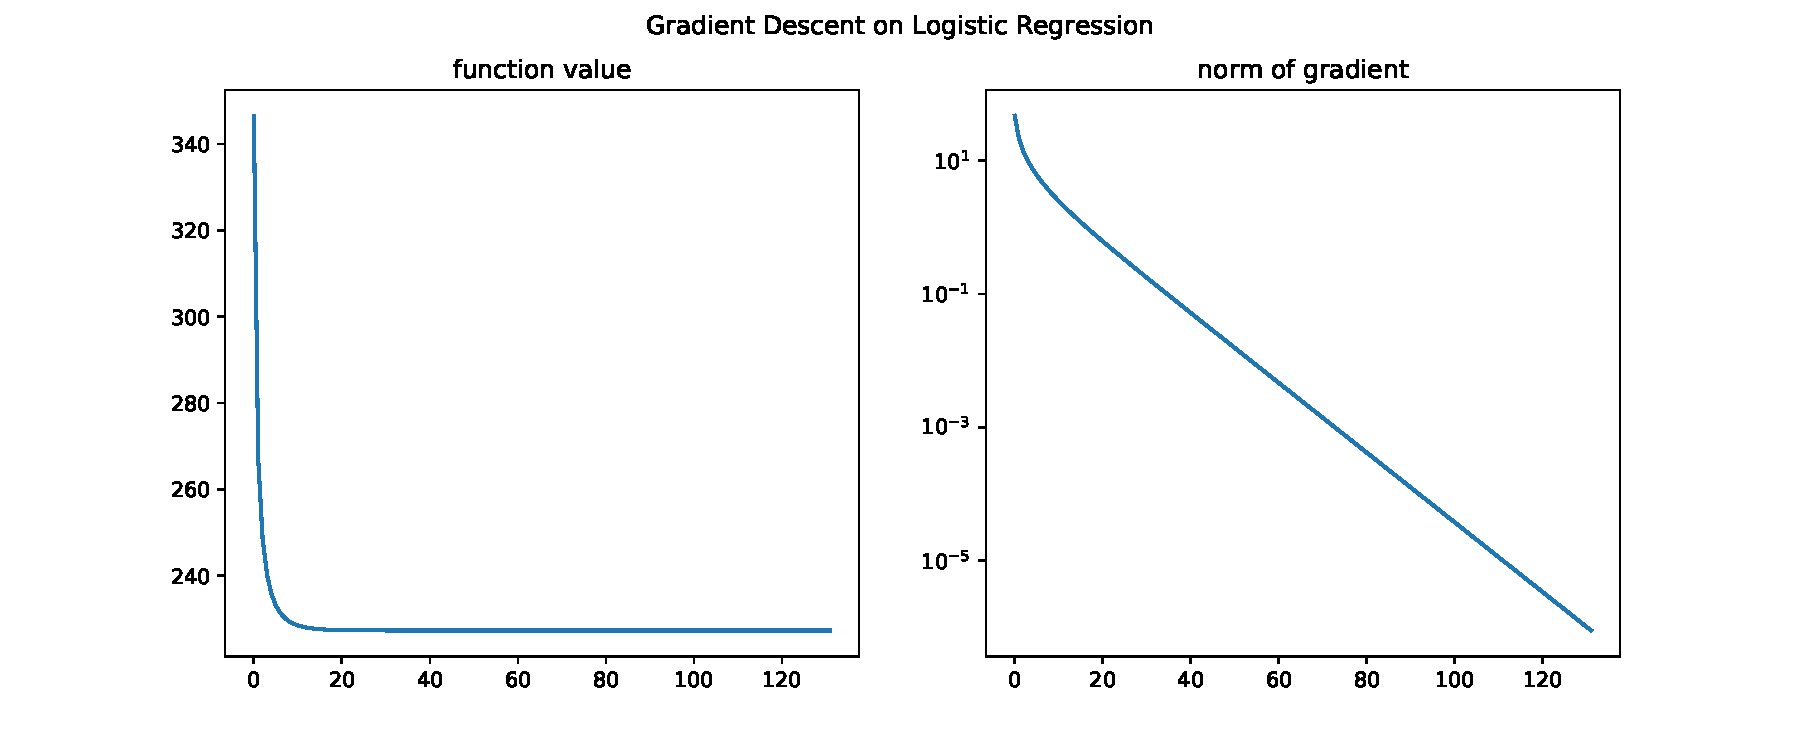
\includegraphics[width=\textwidth]{logistic_gradient_descent.pdf}
  \caption{Gradient descent with a constant step size was used to minimize the
    logistic regression objective on the randomly generated sample data.}
  \label{fig:logistic_gradient_descent}
\end{figure}

See Figure \ref{fig:logistic_gradient_descent}. I used the result in problem
5(b) to choose a constant step size of $\frac{1}{\beta}$.

    
\item Implement Newton's method for the same problem. Does the method converge? If necessary, use the line search routine provided
  to scale your updated directly to ensure descent. Add the plots for Newton's method (a) and (b) to your Figures 1 and 2. What do you notice?

  \begin{figure}
    \centering
    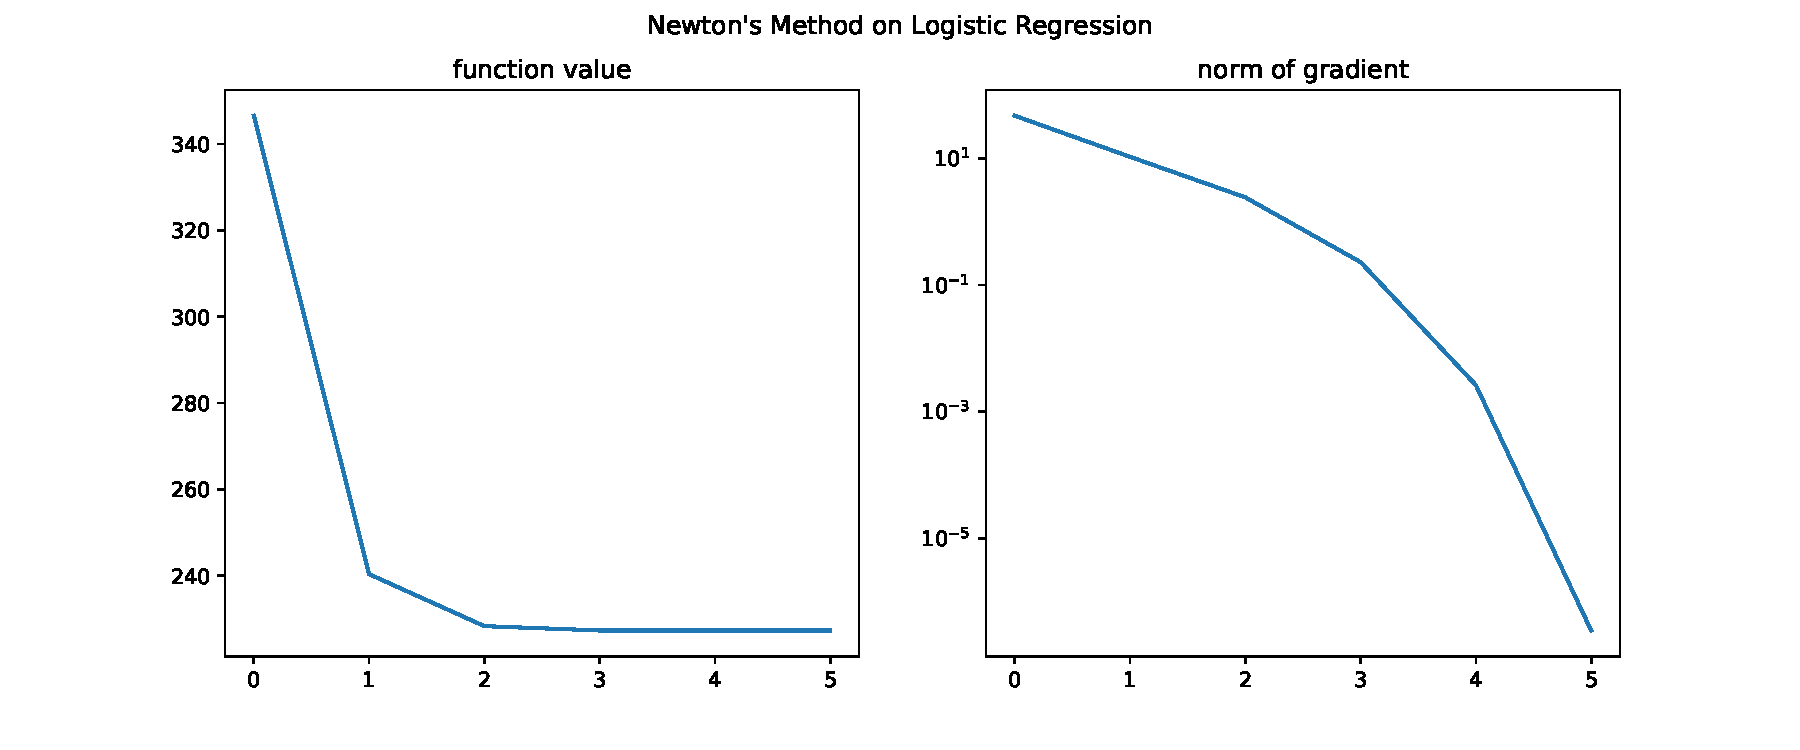
\includegraphics[width=\textwidth]{logistic_newton.pdf}
    \caption{Newton's method used to minimize the logisitic regression objective
      on the randomly generated sample data.}
    \label{fig:logistic_newton}
  \end{figure}

See Figure \ref{fig:logistic_newton}. The method converges much more quickly:
gradient descent takes 131 steps, and Newton's method merely takes 5 steps.
  
\item Using the sample (Poisson) data  and starter code provided, implement gradient descent and Newton's method for $\ell_2$-regularized Poisson regression. You may need to use the line search routine for 
  both algorithms. Make the same plots as you did for the logistic regression examples.

  \begin{figure}
  \centering
  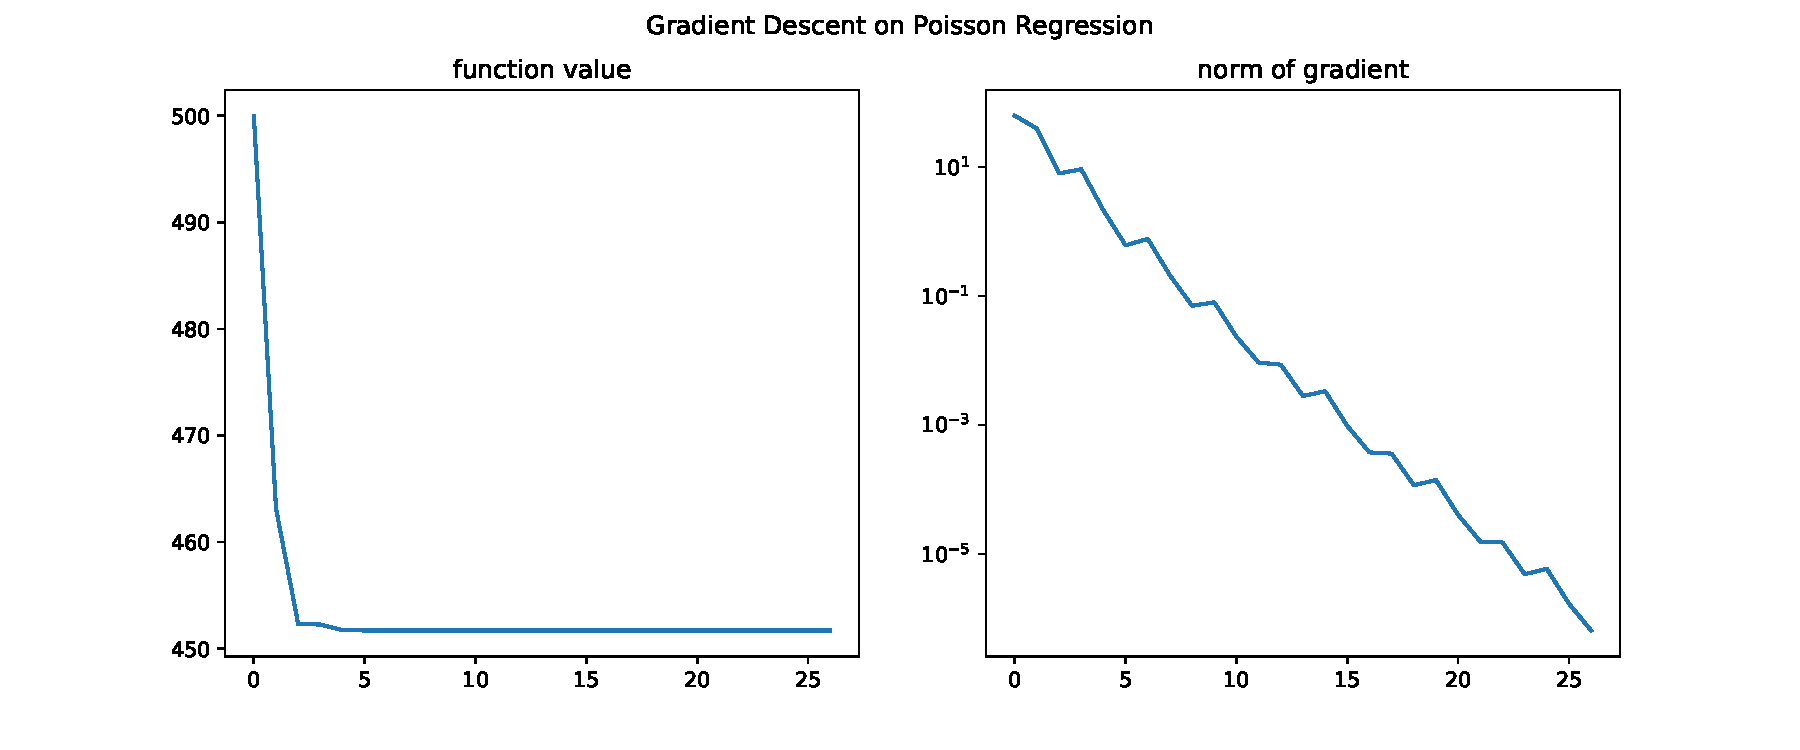
\includegraphics[width=\textwidth]{poisson_gradient_descent.pdf}
  \caption{Gradient descent with line search was used to minimize the Poisson
    regression objective on the randomly generated sample data.}
  \label{fig:poisson_gradient_descent}
\end{figure}

\begin{figure}
  \centering
  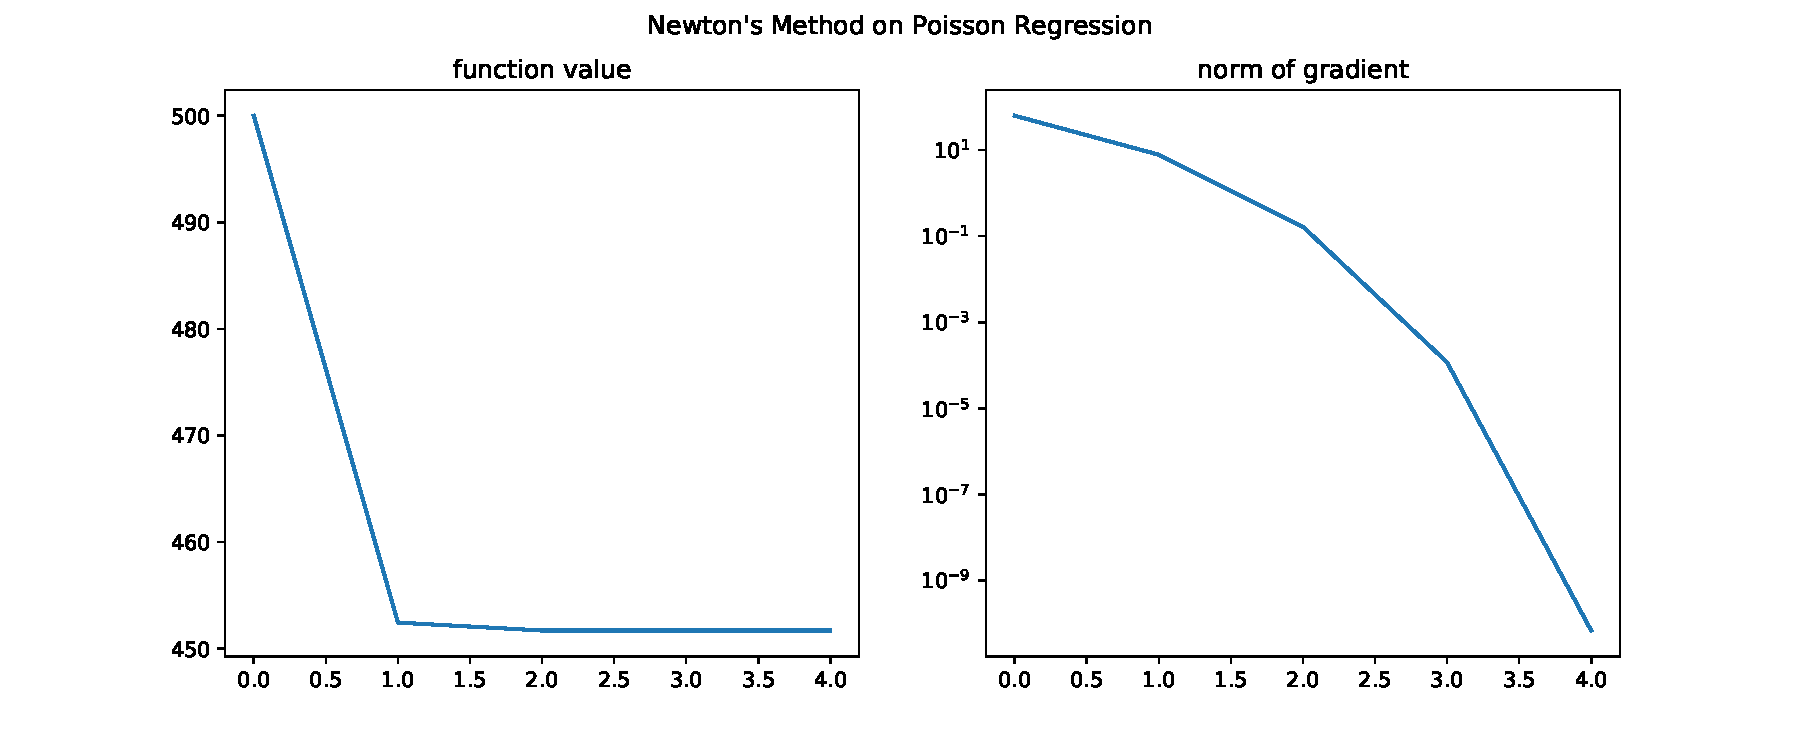
\includegraphics[width=\textwidth]{poisson_newton.pdf}
  \caption{Newton's method used to minimize the Poisson regression objective on
    the randomly generated sample data.}
  \label{fig:poisson_newton}
\end{figure}

See Figures \ref{fig:poisson_gradient_descent} and
\ref{fig:poisson_newton}. Line search was used to determine the step size at
each step in gradient descent.
  
\item What do you notice qualitatively about steepest descent vs. Newton?

  Steepest descent takes many more iterations to converge. In particular, the
  linear rate of convergence is evident in the plots of the gradient norms for
  steepest descent. Likewise, in the plots of the gradient norms for Newton's
  method, we see quadratic rate of convergence as expected. 
\end{enumerate}

\bigskip\bigskip




\end{enumerate}


\end{document}  
